\section{Introducción}

\subsection{Marco contextual}

\begin{frame}{Caja}
   \begin{Block}{Arquitectura de computadoras}
      Disciplina que se encarga de determinar del comportamiento funcional de una computadora desde el punto de vista del programador. Aspectos considerados en esta disciplina son:
   \begin{itemize}
      \item Los tipos de datos y su tamaño
      \item Las operaciones que realiza
   \end{itemize}
   \end{Block}
\end{frame}

\begin{frame}{Dos columnas}
  \begin{twocols}
    \colx{
      \begin{itemize}
        \item item
        \item item
      \end{itemize}
    }
    \coly{
      \centering
      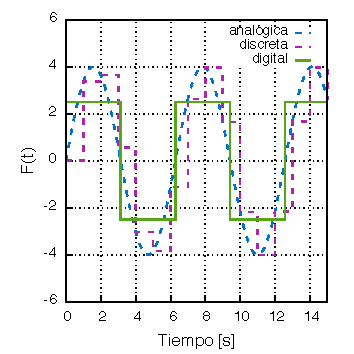
\includegraphics[width = \textwidth]{analog}
    }
  \end{twocols}
\end{frame}


